\documentclass[conference]{IEEEtran}
\IEEEoverridecommandlockouts
% The preceding line is only needed to identify funding in the first footnote. If that is unneeded, please comment it out.
\usepackage{cite}
\usepackage{amsmath,amssymb,amsfonts}
\usepackage[T1]{fontenc}
\usepackage{algorithmic}
\usepackage{amsmath,amssymb,amsfonts}
\usepackage{graphicx}
\usepackage{textcomp}
\usepackage{xcolor}
\usepackage{listings}
\usepackage{hyperref}
\usepackage{subcaption}
\usepackage{caption}
\usepackage{multirow}
\usepackage{float}

\def\BibTeX{{\rm B\kern-.05em{\sc i\kern-.025em b}\kern-.08em
    T\kern-.1667em\lower.7ex\hbox{E}\kern-.125emX}}
\begin{document}

\title{MACHINE LEARNING APPROACH FOR THE PREDICTION OF THE STATUS OF TANZANIAN WELLS [COMP4030 CW2 - Data Science and Machine Learning]
}

\author{\IEEEauthorblockN{*Thomas Cotter}
\IEEEauthorblockA{\textit{Computer Science} \\
\textit{University of Nottingham}\\
Nottingham, England\\
psytc8@nottingham.ac.uk}
\and
\IEEEauthorblockN{*Loo Yang Shen Jason}
\IEEEauthorblockA{\textit{Computer Science} \\
\textit{University of Nottingham}\\
Nottingham, England \\
hfyyl5@nottingham.ac.uk}
}

\maketitle

\begin{abstract}
  This paper details our approaches and results for the COMP4030 CW2. We have used a number of machine learning algorithms in order to predict the status ('Functional', 'Functional - Needs Repair' \& 'Non-Functional') of water wells in Tanzania. This is important as not only does knowing the status of the well help keep the total percentage of functioning wells higher, but it also allows for more effective spending from the government as they no longer would have to send workers out to check the status of the well. Our results suggested that the most important features were \textbf{ADD RESULTS}, and the best classification model as \textbf{ADD RESULTS}
\end{abstract}

\begin{IEEEkeywords}
  Machine Learning, Data Science, Classification
\end{IEEEkeywords}

\section{Introduction}

\subsection{Research Questions}

\textbf{What factors are most important for determining the status of a well, and how accurately can we classify wells based on these features?}. 

We choose this question because we are interested in the factors that determine the status of a well, and using ML to try to classify these wells into 1 of 3 classes: Functional, Non-Functional \& Functional Needs Repair. Follow-up questions to this question could include:
    \begin{itemize}
        \item How does the accuracy of the classification model vary with different feature sets and classification algorithms?
        \item Could we use our results to ensure that wells are built and repaired so that fewer wells are non-functional?
    \end{itemize}

\subsection{Dataset}

The chosen dataset is from the Tanzanian Ministry of Water and contains information on the status of wells in Tanzania. This dataset has 59400 rows, with 40 different features. These 40 features could be broken down into three subgroups: a) Geographic Location of the Wells. b) Management of the wells. and c) Water Condition of the wells. The dataset is originally split into 2 different files, one for labels and one for the actual data. These can be merged easily with pandas through left join on the "ID" column. 

Fig. \ref{fig:status_groups} shows the distribution of the target variable, which is the status of the well. We can see from this that we might need to oversample the 'functional needs repair' class, due to class imbalance.

\begin{figure}[h]
    \centering
    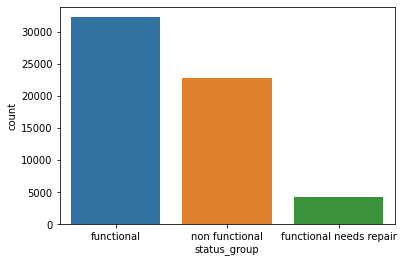
\includegraphics[scale=0.5]{figures/status_groups.png}
    \caption{Distribution of the target variable}
    \label{fig:status_groups}
\end{figure}

\subsection{Management Structure}

A requirement of this project was to work separately within our pairs and try different techniques to solve the problem. In order to not lost important insights, we communicated the our found results periodically. We took the three stages, 'Data Analysis', 'Data Preprocessing' \& 'Data Classification' and followed a 'Chistmas Tree'-like management approach. This means for section, we performed our own analysis, before combining our results and moving onto the next section. This was also done cyclically, for example when we re-examined the Preprocessing step in order to improve classification results. See Fig. \ref{fig:management_structure} for more details

\begin{figure}[h]
    \centering
    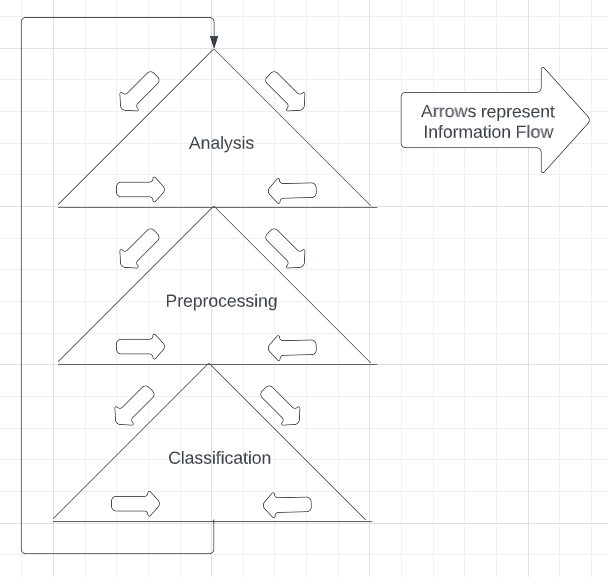
\includegraphics[scale=0.35]{figures/ct_approach.png}
    \caption{Management Structure}
    \label{fig:management_structure}
\end{figure}

This results in a number of benefits. Firstly, it allows us to research a large number of approaches, which provides a higher chance of finding a powerful approach. Secondly, the combination of approaches that resulted might have never happened when working individually, which may provide more optimal results. 

\section{Literature Review}

One study by Pathak et al. (2023) \cite{pathak2023pump} compared the performance of TabNet, a sequential attentive classification architecutre designed for tabular data, and tree-based approaches such as XBBoost. They found that TabNet outpeformed XGBoost, boasting an 83\% accuracy compared to XGBoosts 78\%. TabNet makes use of Transformers, a machine learning algorithm which uses self-attention to differentially weight the significance of each part of the input. A point of note is that TabNet does not require feature engineering to perform at these standards. We have not used TabNet in our report, as our primary goal was to showcase an end-to-end machine learning solution, and this includes feature enginering. However, it provides an interesting comparision.

Pham et al studied fully connected neural networks on the Pump it Up dataset \cite{Pham_2018}, settling on a model with 7 hidden layers and cross-entropy loss as the loss function. Their trained model achieved a 78.6\% accuracy rate on the test dataset. Although our project has prioritized tree-based methods for their speed, it would be interesting to compare our results with those of a neural network.

Jithin Paul also undertook a study on the Pump it Up dataset, experimenting with different models to test for the best results \cite{Paul_2023}. He proposed four methods, RandomForest, DeepLearning, LogisticRegression \& AdaBoost. The results showed that RandomForest, was the most accurate model, achieving a mean accuracy of 81.18\% on the test dataset. This finding demonstrates that tree-based models perform exceptionally well on this dataset, which motivated us to use more sophisticated tree-based methods in our own work.

\section{Methodology}

\subsection{Data Analysis}

When conducting data analysis, the python library Seaborn \cite{seaborn} was our primary data visualization tool. We found that Seaborn produces more visually appealing graphs than those produced by MatPlotLib and the library itself is simpler to use.

\subsubsection{Thomas}

Thomas produced visualizations to determine the correlation between 'construction\_year'and other features in the dataset. This feature had a number of missing values, therefore the objective behind these graphs was to determine the possibility of using other features to impute these missing values.

\subsubsection{Jason}

Jason checked the number of missing and unique values across 38 features provided. The main reasoning behind it was to identify features that would require imputations due to missing or invalid values. In addition, this step allowed him to distinguish features which would have to be recategorised due to the large number of unique values present.  He also generated Count Plots for each of the previously mentioned features based on water wells' status. These plots allowed him to visualise the distribution of the wells' status based on features. Thus, making it easier to identify features that could possibly influence the status of a water well.

\subsection{Data Preprocessing}

\subsubsection{Thomas}

Thomas initially performed the imputation of the latitude \& longitude missing values by applying mean imputation with a specific approach. The data was grouped by 'ward', 'lga' and then 'region'. This ensured that any missing values in either 'ward' or 'lga' did not result in missing lat / lon values. This also provides more accurate results than just 'regular' mean imputation, as the imputed values are localised.

He also looked at the Funder \& Installer columns, which contained 1000s of unique values. In his approach, he decided to group the column into categories: 'Charity', 'Government', 'Local Government', 'Private', 'Religious', 'Foreign', 'School' \& 'Unknown'. This was done to simplify the dataset, making it easier for the model to learn the distribution. Since, the columns had crossover between the values, this can be done in 1 step.

Finally, Thomas also used the SMOTE-ENN algorithm from imblearn \cite{smote-enn}, to balanced the imbalance in the 'Functional - Needs Repair' class. Imbalanced datasets could potentially affect model performance, especially in tree-based models.

Finaly, 'gps-height' was normalised using a custom MinMaxScaler and a custom Z-Score Scaler. This was due to the prevelence of outliers in the 'gps-height' feature.

\subsubsection{Jason}

Due to the presence of missing data in the Latitude \& Longitude columns, Jason decided to apply mean imputation based on the Region column. The values of the Region column corresponds with the name of cities present in Tanzania. By calculating the  mean latitude and longitude value of each region, a rough estimation of the geographical location of wells with missing value could be known. Therefore, allowing valuable insights to be learnt by ML models during training.

During the Data Analysis Phase, he had noticed that two columns Permit and Public Meeting had missing values. Upon further inspection, these two columns only contain the values of either 'True' or 'False'. Data Imputation was not done at this stage due to the lack of valuable data present in the data set. To preserve the distribution of these two columns, a unique values known as 'Unknown' was given to rows with missing data.

Jason had performed data recategorisation on both funder and installer columns which contained 1000 - 2000 unique values. He had first performed data cleaning to fix spelling mistakes that were present in each column. This was followed by identifying unique values with count above the threshold of 1000. Each unique value above the previously mentioned threshold would be classified as its own individual class while those below it would be classified under the 'Other' value. Data recategorisation would be able to reduce the number of unique values present in these two columns leading to better ML model training performance.

Although the number of unique values in the Region Column are minimal, Jason decided to reclassify them according to their geographical zones based on data that was provided by the Tanzania Water and Sanitation Network \cite{tawasanet}. This reduced the number of unique values of the Region Column to 7 from 21. New insights could potentially be drawn upon  based on the zone that the water wells is currently located in.

The data set provided had feature and target variables in the form of categorical form. Jason had converted these features into numerical form that is required of by ML models prior to training. He had encoded the values of the feature and target variables in the form of alphabetical order whereby a = 0, b = 1 etc. 

\subsection{Data Classification}

Initially, our focus was on testing the performance of different algorithms without any feature selection. This would allows us to focus on the best performing ones. The results can be seen in Table. \ref{tab:initial-clf-results}. From these, we can see that XGBoostClassifier, CatBoostClassifier, BaggingClassifier \& HistGradientBoostingClassifier were the most effective for our problem. We decided to explore these models using feature selection \& hyper-parameter tuning. Our feature selection process employed a Chi-Squared test and feature importances obtained from a RandomForest and a XGBoost.

\begin{table}[h]
  \centering
  \caption{Initial Classification Results}
  \label{tab:initial-clf-results}
  \begin{tabular}{|c|c|c|c|}
    \hline
    \textbf{Algorithm} & \textbf{Accuracy} & \textbf{Precision} & \textbf{Recall} \\ \hline
    XGB	& \textbf{0.799} & \textbf{0.751} & 0.633 \\
    \hline
    CatBoost & 0.795 & 0.746 & 0.634 \\
    \hline
    Bagging & 0.793 & 0.704 & \textbf{0.659} \\
    \hline
    HistGradientBoosting & 0.791 & 0.743 & 0.624 \\
    \hline
    DT & 0.757 & 0.643 & 0.645 \\
    \hline
    KNN & 0.709 & 0.623 & 0.563 \\
    \hline
  \end{tabular}
\end{table}


\subsubsection{Thomas}

Thomas trained the 4 top models (XGBoost, CatBoost, Bagging \& HGBoost) on the SMOTE balanced dataset and compared the results to models trained on the imbalanced dataset. The results were also compared when optimizing for 'recall\_macro' or 'accuracy'. The reason for this is that recall is usually a better metric for imbalanced datasets, as accuracy can often misrepresent the truth. 'recall\_macro' takes an average of the recall for all 3 classes, which makes it a good metric to use.

Furthermore, he used Weights and Biases (WandB) \cite{wandb} to analyse the subset of features produced by the Chi-Squared Test and RandomForest.  WandB provided an easy-to-use MLOps platform for tracking our experiments and helped us understand which features worked best for each classifier. He trained multiple classifiers on different subsets of the feature set (ranging from sizes 0.75N to N, where N is the size of the original feature set), and tracked this information in WandB. WandB allows us to quickly filter for the best performing 'runs', and find out which feature set was used in this run. He also used WandB to further analyse the results of his cross-validation hyper-parameter tuning, in much a similar process to feature selection.

\subsubsection{Jason}

From the Random Forest feature importance and Chi-Squared Test, Jason had shortlisted 16 features that influenced the classification of Tanzanian Water Wells. Prior to model training, the dataset was subjected to a 80\%:20\% train test split. This was followed by normalising the testing and training set features with z-score normalisation.

For this study, he considered three different machine learning models  (Random Forrest, XGBoost \& CatBoost). Hyperparameter tuning was conducted via GridSearchCV \cite{gridsearch} from the sklearn library. Upon completion of the hyperparameter tuning process, the most optimal parameters of each model were recorded before being passed for model training. 

To evaluate the performance of each model, Jason used three different evaluation methods. K-fold cross validation with the value of K being 5 , confusion matrix and receiver operating characteristic (ROC) curve. K-fold cross validations was used to evaluate the performance of the model on unseen data. Meanwhile, confusion matrix showcases the predictions which are labelled correctly and incorrectly by class. Although ROC Curve is usually meant for binary classification, it could still be extended to multiclass classification through pairwise comparison i.e., one class vs all other classes.   

\section{Results} \label{ref:results}

\subsection{Data Analysis}

\subsubsection{Thomas}

As mentioned, Thomas produced a number of visualisations to help understand the construction year feature. One example of these can be seen in Fig. \ref{fig:construction_year}. From these, we can see that there is a slight variation in Waterpoint Type usage across decades, but nothing of significance. The same is true across the other visualisations produced (see the accompanying ipynb for more details). For this reason, the missing values in the Construction year were kept as 'Unknown'. The distribution of the status group values within instances with 'Unknown' or 'Not Unknown' construction-year values can be seen in Fig \ref{fig:construction_year}.

\begin{figure*}[t!]
    \centering
    \begin{subfigure}[t]{0.5\textwidth}
      \centering
      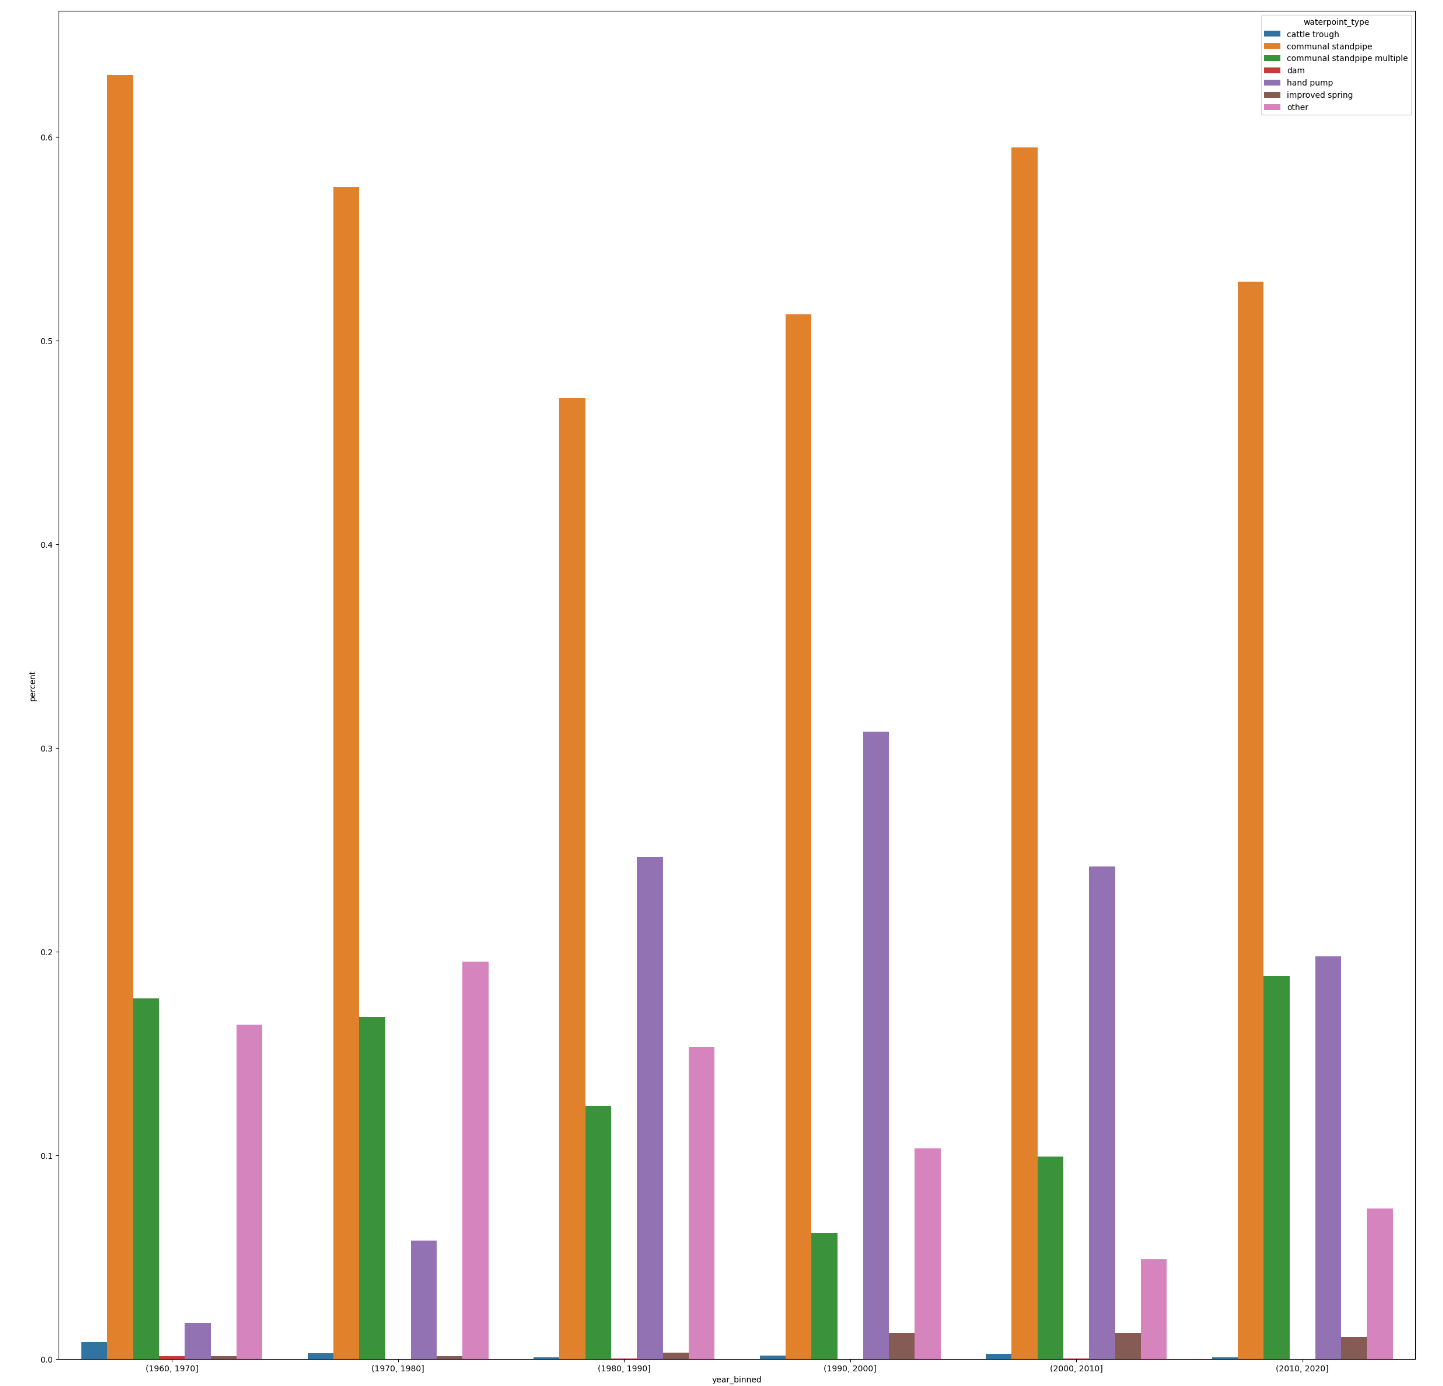
\includegraphics[height=3in]{figures/tom_da_construction_year_1}
      \caption{Waterpoint Type vs Construction Year}
    \end{subfigure}%
    ~
    \begin{subfigure}[t]{0.5\textwidth}
      \centering
      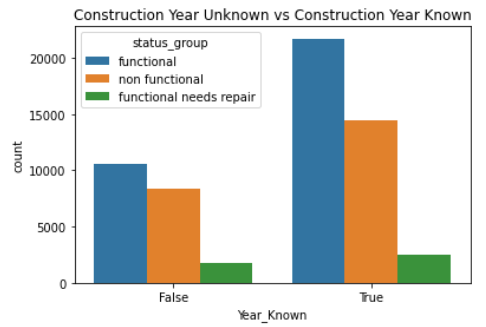
\includegraphics[height=2in]{figures/tom_unknown_cy.png}
      \caption{Construction Year Unknown vs Construction Year Known}
    \end{subfigure}
    ~
    \caption{Construction Year Data Analysis}
    \label{fig:construction_year}
\end{figure*}
    
\subsection{Data Preprocessing}

\subsubsection{Thomas}

Firstly, The results of the latitude and longitude can be seen in Fig. \ref{fig:lat_long_imputation}.

\begin{figure*}[t!]
  \centering
  \begin{subfigure}[t]{0.3\textwidth}
      \centering
      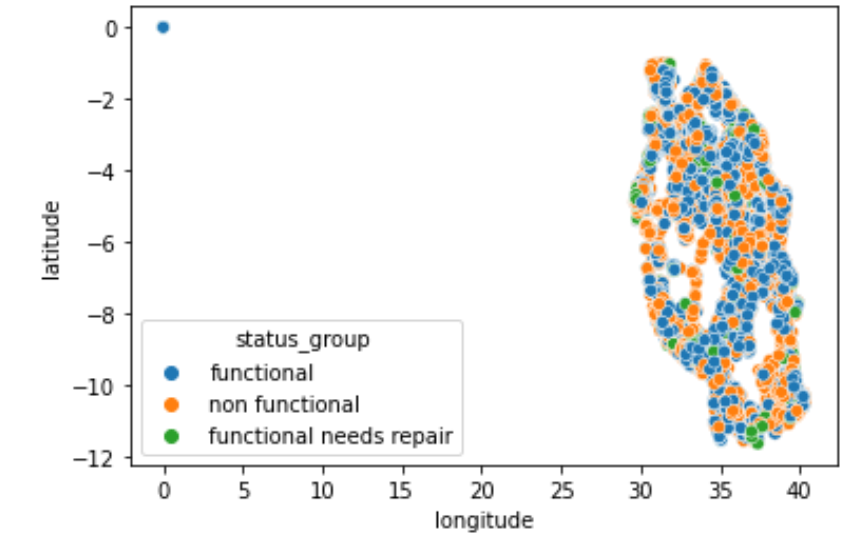
\includegraphics[height=1.45in]{figures/tom_impute_lat_1}
      \caption{Pre-Imputation Latitude \& Longitude}
  \end{subfigure}%
  ~
  \begin{subfigure}[t]{0.3\textwidth}
      \centering
      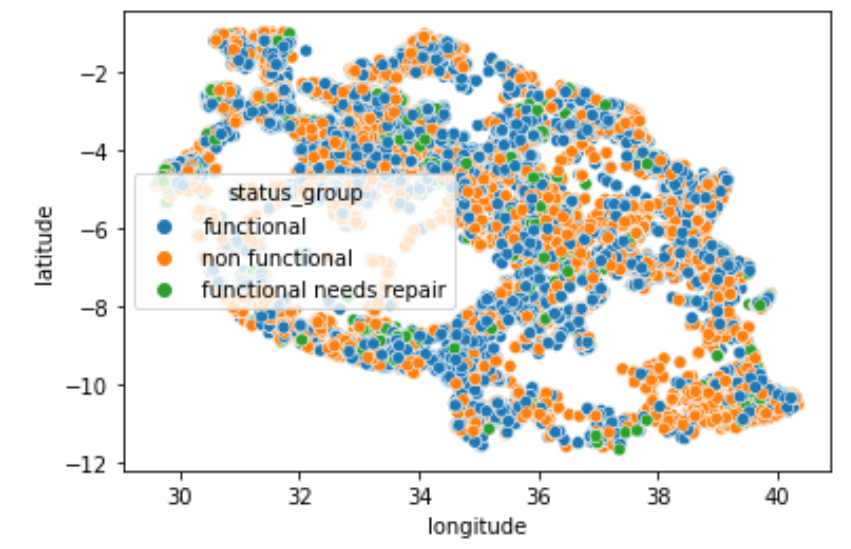
\includegraphics[height=1.5in]{figures/tom_impute_lat_2}
      \caption{Post-Imputation Latitude \& Longitude}
  \end{subfigure}
  ~
  \begin{subfigure}[t]{0.3\textwidth}
      \centering
      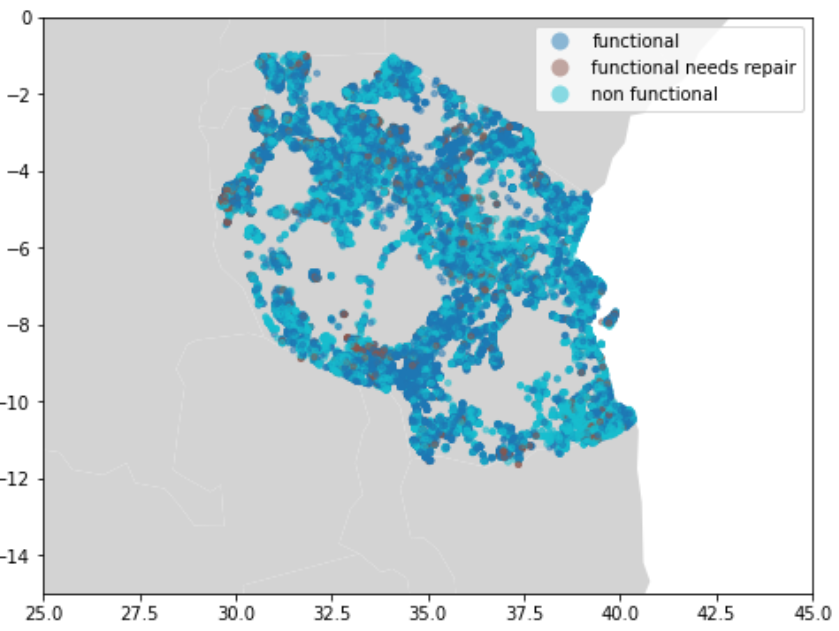
\includegraphics[height=1.5in]{figures/tom_impute_lat_3}
      \caption{Imputated Latitude \& Longitude Overlayed onto a map of Tanzania}
  \end{subfigure}
  ~
  \caption{Latitude \& Longitude Imputation}
  \label{fig:lat_long_imputation}
\end{figure*}

Secondly, as mentioned the installer and funder column were categorized. This was performed manually using Thomas' own knowledge on the subject and the internet. The result was 8 categories, the counts for each of those categories in both the Funder \& Installer column can be seen in Table \ref{tab:funder_installer_categories}. These categorized versions of the features proved to provide some benefit to the model when testing the subset of features to use in WandB.

\begin{table}[h]
  \centering
  \caption{Funder \& Installer Categories}
  \label{tab:funder_installer_categories}
  \begin{tabular}{|c|c|c|}
    \hline
    Column & Category & Count \\
    \hline
    \multirow{8}{*}{Funder} & Government & 20199 \\
    & Charity & 11066 \\
    & Unknown & 8216 \\
    & Foreign Aid & 8131 \\
    & Religious & 4087 \\
    & Private & 3889 \\
    & Local Government & 3774 \\
    & School & 38 \\
    \hline
    \multirow{8}{*}{Installer} & Local Government & 22515 \\
    & Government & 10327 \\
    & Unknown & 8800 \\
    & Charity & 7487 \\
    & Private & 3853 \\
    & Foreign Aid & 3346 \\
    & Religious & 3046 \\
    & School & 26 \\
    \hline
  \end{tabular}
\end{table}

Finally, Thomas used the SMOTE-ENN algorithm to oversample the minority class. The results of this can be seen in Fig. \ref{fig:smote}. In this figure, O is 'Functional', '1' is 'Functional - Needs Repair' and 2 is 'Non-Functional'. 

\begin{figure*}[t!]
  \centering
  \begin{subfigure}[t]{0.5\textwidth}
      \centering
      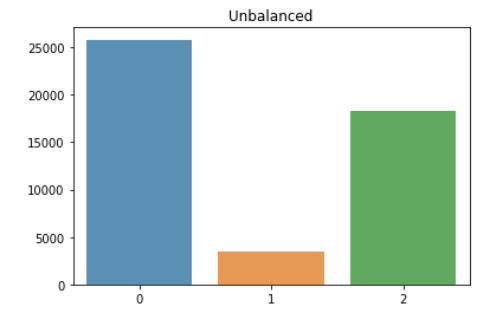
\includegraphics[height=2.25in]{figures/tom_smote_1}
      \caption{Pre-Oversampling Class Distribution}
  \end{subfigure}%
  ~
  \begin{subfigure}[t]{0.5\textwidth}
      \centering
      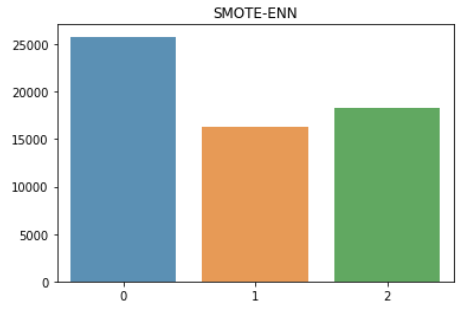
\includegraphics[height=2.25in]{figures/tom_smote_2}
      \caption{Post-Oversampling Class Distribution}
  \end{subfigure}
  ~
  \caption{SMOTE-ENN Oversampling}
  \label{fig:smote}
\end{figure*}

\subsection{Classification} \label{ref:classification_results}

\subsubsection{Thomas}

Post hyper-parameter tuning, metrics including accuracy, precision ('macro'), recall ('macro') and f1-score were calculated for each of the models. The models were tested on both the imbalanced and SMOTE-ENN balanced dataset. The results can be seen in Table \ref{tab:classification_results}

\begin{table*}[t]
  \centering
  \caption{Classification Results}
  \label{tab:classification_results}
  \begin{tabular}{|c|c|c|c|c|c|c|}
    \hline
    \textbf{Scoring} & \textbf{Dataset} & \textbf{Model} & \textbf{Accuracy} & \textbf{Precision} & \textbf{Recall} & \textbf{F1-Score} \\
    \hline
    \multirow{2}{*}{Recall Macro} & \multirow{4}{*}{Balanced} & XGBoost & 0.802 & 0.701 & 0.668 & 0.683 \\
    & & CatBoost & 0.783 & 0.669 & 0.660 & 0.664 \\
    & & HistGradientBoosting & 0.796 & 0.693 & 0.665 & 0.677 \\
    & & BaggingClassifier & 0.803 & 0.703 & \textbf{0.676} & \textbf{0.687} \\
    \cline{2-7}
    & \multirow{4}{*}{Imbalanced} & XGBoost & 0.804 & 0.720 & 0.662 & 0.683 \\
    & & CatBoost & 0.791 & 0.697 & 0.652 & 0.668 \\
    & & HistGradientBoosting & 0.806 & 0.730 & 0.658 & 0.681 \\
    & & BaggingClassifier & 0.803 & 0.722 & 0.660 & 0.681 \\
    \hline
    \multirow{2}{*}{Accuracy} & \multirow{4}{*}{Balanced} & XGBoost & 0.800 & 0.700 & 0.662 &  0.677 \\
    & & CatBoost & 0.787 & 0.678 & 0.665 & 0.670 \\
    & & HistGradientBoosting & 0.797 & 0.699 & 0.666 & 0.680 \\
    & & BaggingClassifier & 0.801 & 0.701 & 0.671 & 0.684 \\
    \cline{2-7}
    & \multirow{4}{*}{Imbalanced} & XGBoost & 0.804 & \textbf{0.748} & 0.648 & 0.676 \\
    & & CatBoost & 0.797 & 0.753 & 0.635 & 0.665\\
    & & HistGradientBoosting & 0.806 & 0.733 & 0.662 & 0.686 \\
    & & BaggingClassifier & \textbf{0.811} & 0.741 & 0.656 & 0.681 \\
    \hline
  \end{tabular}
\end{table*}

From these results, we can see that although the difference in minimal, the BaggingClassifier performs the best. The balanced dataset provides a slight increase in F1-Score, yet accuracy is better with the imbalanced dataset. This makes sense, as incorrectly classifying the minority class has a small impact on accuracy but a large impact on F1-Score.

Thomas also produced the two confusion matrices, as seen in Fig. \ref{fig:confusion_matrices}. These were produced by a XGBoost, and show the output of training on both the balanced and imbalanced datasets. We can see from these matrics that balancing the dataset results in less False Positives. If the goal of your model was to do specifically this, perhaps using the balanced dataset would be the best idea. This was not the case for us, so we continued with using the imbalanced dataset.

\begin{figure*}
  \centering
  \begin{subfigure}[t]{0.5\textwidth}
      \centering
      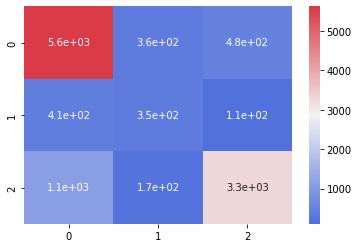
\includegraphics[height=2.25in]{figures/cm_balanced}
      \caption{Balanced Dataset}
  \end{subfigure}%
  ~
  \begin{subfigure}[t]{0.5\textwidth}
      \centering
      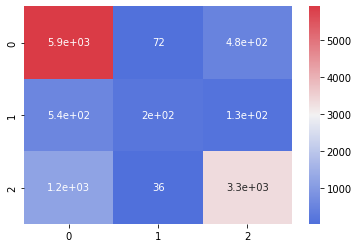
\includegraphics[height=2.25in]{figures/cm_imbalanced}
      \caption{Imbalanced Dataset}
  \end{subfigure}
  ~
  \caption{Balanced vs Imbalanced Confusion Matrices (XGBoost)}
  \label{fig:confusion_matrices}
\end{figure*}


Since the difference between different models and datasets is neglible, Thomas decided to combine all the models to create a VotingClassifier to possibly squeeze out some extra performance. These results can be seen in Table \ref{tab:voting_classification_results}

\begin{table}[H]
  \centering
  \caption{Voting Classifier Results}
  \label{tab:voting_classification_results}
  \begin{tabular}{|c|c|c|c|}
    \hline
    Accuracy & Precision & Recall & F1-Score \\
    \hline
    0.810 & 0.759 & 0.650 & 0.679 \\
    \hline
  \end{tabular}
\end{table}

Using both the results from model based feature selection, and feature selection after looking at the results from Weights \& Biases, Thomas decided to use the following features in his final model: \textbf{'age'}, \textbf{'latitude\_imputation'}, \textbf{'longitude\_imputation'}, \textbf{'construction\_decade'}, \textbf{'quality\_group'}, \textbf{'basin'}, \textbf{'extraction\_type'}, \textbf{'cat\_installer'}, \textbf{'population'}, \textbf{'gps\_height\_zscorenormalise'}, \textbf{'cat\_funder'}, \textbf{'quantity'}, \textbf{'consistent\_water'}, \textbf{'source\_class'}, \textbf{'zones'}, \textbf{'waterpoint\_type'}, \textbf{'season'}, \textbf{'extraction\_type\_class'}, \textbf{'payment'} (Please consult the ipynb for more details on what information these features contain).

To relate this back to our research questions, we can say that these features are the most important when looking at whether wells are functional or not.We can also say we can classify whether a well is function or not with 81\% accuracy.


\section{Discussion}

In this section, we discuss the results of our analysis. We compare each of our separate approaches to each other, as well as comparing them to the performance of models in the literature.

\subsection{Pre-Processing}

\subsubsection{Tom}

Myself and Jason used many different approaches throughout the project. One example of this is his use of a StandardScaler. He scaled every feature by removing the mean and sacling to a unit variance. I did not scale any features except 'gps\_height', and even then I used a MinMaxScaler. This is an interesting choice considering some of the data is categorical, and yet still produced quality results. Another difference in pre-processing was the handling of the funder and installer columns. We both took different approaches to this, and in my opinion Jason's technique proved slightly better. By categorizing the entire dataset, valuable information was lost was looking at the specific funders or installers, the information lost in Jason's technique was smaller as only values with small counts were removed from the dataset and classified as 'Other'.


\subsection{Modelling}

\subsubsection{Tom}

We also used different hyper-parameter tuning methods, specifically GridSearch (Jason) and RandomSearch (Tom). The RandomSearch is faster and allowed me to research and test a wider range of hyper-parameters for a wider range of models. However, the GridSearch is in a sense more 'deep', focusing in on potential hyper-parameters that could be good. I think this is reflected in our results, as Jason's XGBoost slightly out-performed my XGBoost on the test set, however the breadth of search allowed me to find the BaggingClassifier, which performed very well. 

\subsection{Literature Discussion}

When comparing to the TabNet implementation by Pathak et al \cite{pathak2023pump}, we can see that our best classifiers were out-performed by TabNet by at least 2\%. This is quite significant. It's understandable that this is the case due to the capabilities of Transformers. 

We also reviewed Pham et al \cite{Pham_2018} and found that their produced Neural Network (NN) was not as high performing as some more lightweight models. XGBoost / HistGradientBoost and BaggingClassifier all out-perform the NN. These lightweight models also are much faster to train than an NN, so it is much more efficient to use these models on a dataset such as Pump It Up.

\section{Conclusion}

\bibliographystyle{IEEEtran}
\bibliography{refs}

\end{document}


